%https://latexdraw.com/draw-flowcharts-latex-tutorial/

%https://tex.stackexchange.com/questions/8890/tikz-how-to-draw-boxes-around-set-of-nodes

%https://tikz.dev/tikz-shapes

%https://tex.stackexchange.com/questions/8890/tikz-how-to-draw-boxes-around-set-of-nodes

%https://www.latex4technics.com/?note=189T

\documentclass[border=0.2cm]{standalone}
 
% Required packages
\usepackage{comment}
\usepackage{tikz}
\usetikzlibrary{shapes,positioning,calc}


\usepackage{color}
\definecolor{franklinblue}{RGB}{0,43,83}
\definecolor{cardinalred}{RGB}{140,21,21}
\definecolor{skobeloff}{rgb}{0.0, 0.48, 0.45}
\definecolor{auburn}{rgb}{0.43, 0.21, 0.1}
\definecolor{calpolypomonagreen}{rgb}{0.12, 0.3, 0.17}
\definecolor{ao(english)}{rgb}{0.0, 0.5, 0.0}

\tikzset{
    ncbar angle/.initial=90,
    ncbar/.style={
        to path=(\tikztostart)
        -- ($(\tikztostart)!#1!\pgfkeysvalueof{/tikz/ncbar angle}:(\tikztotarget)$)
        -- ($(\tikztotarget)!($(\tikztostart)!#1!\pgfkeysvalueof{/tikz/ncbar angle}:(\tikztotarget)$)!\pgfkeysvalueof{/tikz/ncbar angle}:(\tikztostart)$)
        -- (\tikztotarget)
    },
    ncbar/.default=0.5cm,
}
\tikzset{square left brace/.style={ncbar=0.5cm}}
\tikzset{square right brace/.style={ncbar=-0.5cm}}
 
\begin{document}
 
 %https://www.sciencebuddies.org/science-fair-projects/science-fair/steps-of-the-scientific-method

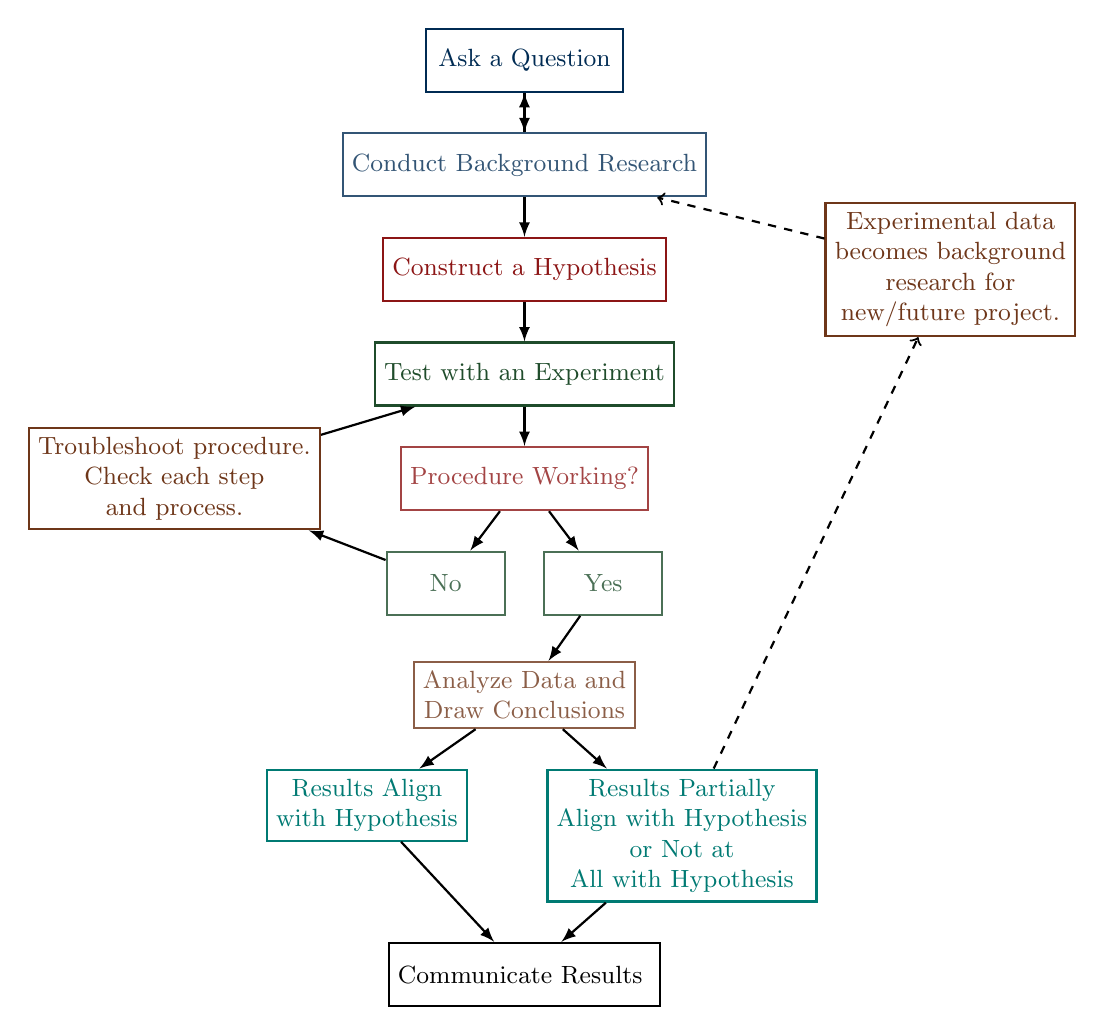
\begin{tikzpicture}[font=\small,thick,align=center]
 
% Start block - Ask a Question
\node[draw=franklinblue,
    text=franklinblue,
    rectangle,
    minimum width=2.5cm,
    minimum height=0.8cm] (block1) {Ask a Question};

% Conduct Background Research
\node[draw=franklinblue!80,
    text=franklinblue!80,
    rectangle,
    below=of block1,
    yshift=0.5cm,
    minimum width=2.5cm,
    minimum height=0.8cm] (block2) {Conduct Background Research};

% Construct a Hypothesis
\node[draw=cardinalred,
    text=cardinalred,
    rectangle,
    below=of block2,
    yshift=0.5cm,
    minimum width=2.5cm,
    minimum height=0.8cm] (block3) {Construct a Hypothesis};

% Test with an Experiment
\node[draw=calpolypomonagreen,
    text=calpolypomonagreen,
    rectangle,
    below=of block3,
    yshift=0.5cm,
    minimum width=2.5cm,
    minimum height=0.8cm] (block4) {Test with an Experiment};   

% Procedure Working
\node[draw=cardinalred!80,
    text=cardinalred!80,
    rectangle,
    below=of block4,
    yshift=0.5cm,
    minimum width=2.5cm,
    minimum height=0.8cm] (block5) {Procedure Working?}; 

% Procedure Working - No
\node[draw=calpolypomonagreen!80,
    text=calpolypomonagreen!80,
    rectangle,
    below=of block5,
    xshift=-1cm,
    yshift=0.5cm,
    minimum width=1.5cm,
    minimum height=0.8cm] (block6) {No};     

% Troubleshoot
\node[draw=auburn,
    text=auburn,
    rectangle,
    left=of block5,
    minimum width=2.5cm,
    minimum height=0.8cm] (blockA) {Troubleshoot procedure. \\ Check each step \\ and process.};  

% Procedure Working - Yes
\node[draw=calpolypomonagreen!80,
    text=calpolypomonagreen!80,
    rectangle,
    below=of block5,
    xshift=1cm,
    yshift=0.5cm,
    minimum width=1.5cm,
    minimum height=0.8cm] (block7) {Yes};

% Experimental data becomes background research for new/future project.
\node[draw=auburn,
    text=auburn,
    rectangle,
    right=of block3,
    xshift=1cm,
    minimum width=2.5cm,
    minimum height=0.8cm] (blockB) {Experimental data \\ becomes background \\research for \\ new/future project.};  

% Analyze Data and Draw Conclusions
\node[draw=auburn!80,
    text=auburn!80,
    rectangle,
    below=of block5,
    yshift=-0.9cm,
    minimum width=1.5cm,
    minimum height=0.8cm] (block8) {Analyze Data and \\ Draw Conclusions};

% Results Align with Hypothesis
\node[draw=skobeloff,
    text=skobeloff,
    rectangle,
    below=of block8,
    xshift=-2cm,
    yshift=0.5cm,
    minimum width=1.5cm,
    minimum height=0.8cm] (block9) {Results Align \\ with Hypothesis};  

% Results Partially Align with Hypothesis or Not al All with Hypothesis 
\node[draw=skobeloff,
    text=skobeloff,
    rectangle,
    below=of block8,
    xshift=2cm,
    yshift=0.5cm,
    minimum width=1.5cm,
    minimum height=0.8cm] (block10) {Results Partially \\Align with Hypothesis \\or Not at \\ All with Hypothesis};

% Communicate Results 
\node[draw=black,
    text=black,
    rectangle,
    below=of block8,
    yshift=-1.7cm,
    minimum width=1.5cm,
    minimum height=0.8cm] (block11) {Communicate Results };

% Arrows
\draw[-latex] (block1) edge (block2)
    (block2) edge (block1)
    (block2) edge (block3)
    (block3) edge (block4)
    (block4) edge (block5)
    (block5) edge (block6)
    (block5) edge (block7)
    (block6) edge (blockA)
    (blockA) edge (block4)
    (block7) edge (block8)
    (block8) edge (block9)
    (block8) edge (block10)
    (block9) edge (block11)
    (block10) edge (block11)
%    (block10) edge (blockB)
%    (blockB) edge (block2)
    ;

\path [black, dashed, ->] (block10) edge node {} (blockB);
\path [black, dashed, ->] (blockB) edge node {} (block2);

\end{tikzpicture}
 
\end{document}